% Created by tikzDevice version 0.10.1 on 2018-01-23 16:20:18
% !TEX encoding = UTF-8 Unicode
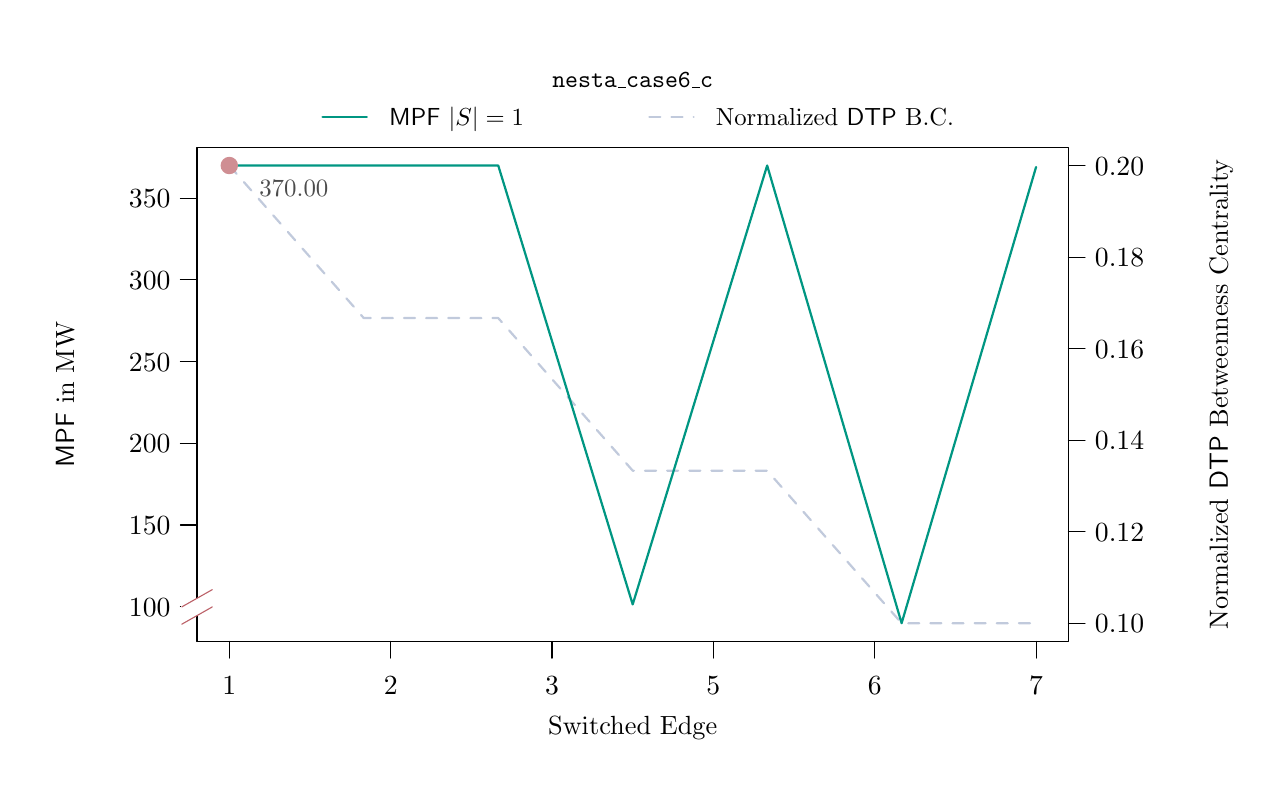
\begin{tikzpicture}[x=1pt,y=1pt]
\definecolor{fillColor}{RGB}{255,255,255}
\path[use as bounding box,fill=fillColor,fill opacity=0.00] (0,0) rectangle (440.85,271.01);
\begin{scope}
\path[clip] (  0.00,  0.00) rectangle (440.85,271.01);
\definecolor{drawColor}{RGB}{193,202,220}

\path[draw=drawColor,line width= 0.8pt,dash pattern=on 4pt off 4pt ,line join=round,line cap=round] ( 72.86,221.20) --
	(121.45,166.07) --
	(170.04,166.07) --
	(218.62,110.94) --
	(267.21,110.94) --
	(315.80, 55.82) --
	(364.39, 55.82);
\end{scope}
\begin{scope}
\path[clip] (  0.00,  0.00) rectangle (440.85,271.01);
\definecolor{drawColor}{RGB}{0,0,0}

\path[draw=drawColor,line width= 0.4pt,line join=round,line cap=round] ( 61.20, 49.20) --
	(376.05, 49.20) --
	(376.05,227.81) --
	( 61.20,227.81) --
	( 61.20, 49.20);
\end{scope}
\begin{scope}
\path[clip] (  0.00,  0.00) rectangle (440.85,271.01);
\definecolor{drawColor}{RGB}{0,0,0}

\path[draw=drawColor,line width= 0.4pt,line join=round,line cap=round] (376.05, 55.82) -- (376.05,221.20);

\path[draw=drawColor,line width= 0.4pt,line join=round,line cap=round] (376.05, 55.82) -- (382.05, 55.82);

\path[draw=drawColor,line width= 0.4pt,line join=round,line cap=round] (376.05, 88.89) -- (382.05, 88.89);

\path[draw=drawColor,line width= 0.4pt,line join=round,line cap=round] (376.05,121.97) -- (382.05,121.97);

\path[draw=drawColor,line width= 0.4pt,line join=round,line cap=round] (376.05,155.04) -- (382.05,155.04);

\path[draw=drawColor,line width= 0.4pt,line join=round,line cap=round] (376.05,188.12) -- (382.05,188.12);

\path[draw=drawColor,line width= 0.4pt,line join=round,line cap=round] (376.05,221.20) -- (382.05,221.20);

\node[text=drawColor,anchor=base west,inner sep=0pt, outer sep=0pt, scale=  1.00] at (385.65, 52.37) {0.10};

\node[text=drawColor,anchor=base west,inner sep=0pt, outer sep=0pt, scale=  1.00] at (385.65, 85.45) {0.12};

\node[text=drawColor,anchor=base west,inner sep=0pt, outer sep=0pt, scale=  1.00] at (385.65,118.52) {0.14};

\node[text=drawColor,anchor=base west,inner sep=0pt, outer sep=0pt, scale=  1.00] at (385.65,151.60) {0.16};

\node[text=drawColor,anchor=base west,inner sep=0pt, outer sep=0pt, scale=  1.00] at (385.65,184.68) {0.18};

\node[text=drawColor,anchor=base west,inner sep=0pt, outer sep=0pt, scale=  1.00] at (385.65,217.75) {0.20};
\end{scope}
\begin{scope}
\path[clip] (  0.00,  0.00) rectangle (440.85,271.01);
\definecolor{drawColor}{RGB}{0,150,130}

\path[draw=drawColor,line width= 0.8pt,line join=round,line cap=round] (106.55,238.60) -- (122.57,238.60);
\definecolor{drawColor}{RGB}{193,202,220}

\path[draw=drawColor,line width= 0.8pt,dash pattern=on 4pt off 4pt ,line join=round,line cap=round] (224.63,238.60) -- (240.65,238.60);
\definecolor{drawColor}{RGB}{0,0,0}

\node[text=drawColor,anchor=base,inner sep=0pt, outer sep=0pt, scale=  0.89] at (218.62,249.28) {\texttt{nesta\_case6\_c}};

\node[text=drawColor,anchor=base west,inner sep=0pt, outer sep=0pt, scale=  0.89] at (130.58,235.54) {$\mathsf{MPF}~|S|=1$};

\node[text=drawColor,anchor=base west,inner sep=0pt, outer sep=0pt, scale=  0.89] at (248.66,235.54) {Normalized~$\mathsf{DTP}$~B.C.};
\end{scope}
\begin{scope}
\path[clip] (  0.00,  0.00) rectangle (440.85,271.01);
\definecolor{drawColor}{RGB}{0,0,0}

\path[draw=drawColor,line width= 0.4pt,line join=round,line cap=round] ( 61.20, 61.79) -- ( 61.20,209.39);

\path[draw=drawColor,line width= 0.4pt,line join=round,line cap=round] ( 61.20, 61.79) -- ( 55.20, 61.79);

\path[draw=drawColor,line width= 0.4pt,line join=round,line cap=round] ( 61.20, 91.31) -- ( 55.20, 91.31);

\path[draw=drawColor,line width= 0.4pt,line join=round,line cap=round] ( 61.20,120.83) -- ( 55.20,120.83);

\path[draw=drawColor,line width= 0.4pt,line join=round,line cap=round] ( 61.20,150.35) -- ( 55.20,150.35);

\path[draw=drawColor,line width= 0.4pt,line join=round,line cap=round] ( 61.20,179.87) -- ( 55.20,179.87);

\path[draw=drawColor,line width= 0.4pt,line join=round,line cap=round] ( 61.20,209.39) -- ( 55.20,209.39);

\node[text=drawColor,anchor=base east,inner sep=0pt, outer sep=0pt, scale=  1.00] at ( 51.60, 58.34) {100};

\node[text=drawColor,anchor=base east,inner sep=0pt, outer sep=0pt, scale=  1.00] at ( 51.60, 87.86) {150};

\node[text=drawColor,anchor=base east,inner sep=0pt, outer sep=0pt, scale=  1.00] at ( 51.60,117.38) {200};

\node[text=drawColor,anchor=base east,inner sep=0pt, outer sep=0pt, scale=  1.00] at ( 51.60,146.90) {250};

\node[text=drawColor,anchor=base east,inner sep=0pt, outer sep=0pt, scale=  1.00] at ( 51.60,176.43) {300};

\node[text=drawColor,anchor=base east,inner sep=0pt, outer sep=0pt, scale=  1.00] at ( 51.60,205.95) {350};
\end{scope}
\begin{scope}
\path[clip] (  0.00,  0.00) rectangle (440.85,271.01);
\definecolor{drawColor}{RGB}{255,255,255}
\definecolor{fillColor}{RGB}{255,255,255}

\path[draw=drawColor,line width= 0.4pt,line join=round,line cap=round,fill=fillColor] ( 55.69, 58.58) rectangle ( 66.71, 64.83);
\definecolor{drawColor}{RGB}{188,97,104}

\path[draw=drawColor,line width= 0.4pt,line join=round,line cap=round] ( 55.69, 55.45) -- ( 66.71, 61.70);

\path[draw=drawColor,line width= 0.4pt,line join=round,line cap=round] ( 55.69, 61.70) -- ( 66.71, 67.95);
\end{scope}
\begin{scope}
\path[clip] ( 61.20, 49.20) rectangle (376.05,227.81);
\definecolor{drawColor}{RGB}{0,150,130}

\path[draw=drawColor,line width= 0.8pt,line join=round,line cap=round] ( 72.86,221.20) --
	(121.45,221.20) --
	(170.04,221.20) --
	(218.62, 62.60) --
	(267.21,221.20) --
	(315.80, 55.82) --
	(364.39,220.67);
\end{scope}
\begin{scope}
\path[clip] ( 61.20, 49.20) rectangle (376.05,227.81);
\definecolor{fillColor}{RGB}{207,142,147}

\path[fill=fillColor] ( 72.86,221.20) circle (  3.15);
\end{scope}
\begin{scope}
\path[clip] ( 61.20, 49.20) rectangle (376.05,227.81);
\definecolor{drawColor}{gray}{0.30}

\node[text=drawColor,anchor=base,inner sep=0pt, outer sep=0pt, scale=  0.90] at ( 96.18,210.04) {370.00};
\end{scope}
\begin{scope}
\path[clip] (  0.00,  0.00) rectangle (440.85,271.01);
\definecolor{drawColor}{RGB}{0,0,0}

\path[draw=drawColor,line width= 0.4pt,line join=round,line cap=round] ( 72.86, 49.20) -- (364.39, 49.20);

\path[draw=drawColor,line width= 0.4pt,line join=round,line cap=round] ( 72.86, 49.20) -- ( 72.86, 43.20);

\path[draw=drawColor,line width= 0.4pt,line join=round,line cap=round] (131.17, 49.20) -- (131.17, 43.20);

\path[draw=drawColor,line width= 0.4pt,line join=round,line cap=round] (189.47, 49.20) -- (189.47, 43.20);

\path[draw=drawColor,line width= 0.4pt,line join=round,line cap=round] (247.78, 49.20) -- (247.78, 43.20);

\path[draw=drawColor,line width= 0.4pt,line join=round,line cap=round] (306.08, 49.20) -- (306.08, 43.20);

\path[draw=drawColor,line width= 0.4pt,line join=round,line cap=round] (364.39, 49.20) -- (364.39, 43.20);

\node[text=drawColor,anchor=base,inner sep=0pt, outer sep=0pt, scale=  1.00] at ( 72.86, 30.00) {1};

\node[text=drawColor,anchor=base,inner sep=0pt, outer sep=0pt, scale=  1.00] at (131.17, 30.00) {2};

\node[text=drawColor,anchor=base,inner sep=0pt, outer sep=0pt, scale=  1.00] at (189.47, 30.00) {3};

\node[text=drawColor,anchor=base,inner sep=0pt, outer sep=0pt, scale=  1.00] at (247.78, 30.00) {5};

\node[text=drawColor,anchor=base,inner sep=0pt, outer sep=0pt, scale=  1.00] at (306.08, 30.00) {6};

\node[text=drawColor,anchor=base,inner sep=0pt, outer sep=0pt, scale=  1.00] at (364.39, 30.00) {7};

\node[text=drawColor,anchor=base,inner sep=0pt, outer sep=0pt, scale=  0.95] at (218.62, 15.60) {Switched Edge};

\node[text=drawColor,rotate= 90.00,anchor=base,inner sep=0pt, outer sep=0pt, scale=  0.95] at ( 16.80,138.51) {$\mathsf{MPF}$ in~$\mathrm{MW}$};

\node[text=drawColor,rotate= 90.00,anchor=base,inner sep=0pt, outer sep=0pt, scale=  0.95] at (433.65,138.51) {Normalized~$\mathsf{DTP}$ Betweenness Centrality};
\end{scope}
\end{tikzpicture}
